\documentclass[12pt,twocolumn,letterpaper]{article}

\usepackage{cvpr}
\usepackage{times}
\usepackage{epsfig}
\usepackage{graphicx}
\usepackage{amsmath}
\usepackage{amssymb}
\usepackage[breaklinks=true,bookmarks=false]{hyperref}
\usepackage{subcaption}

\cvprfinalcopy

\def\httilde{\mbox{\tt\raisebox{-.5ex}{\symbol{126}}}}


\setcounter{page}{1}
\begin{document}

\title{3D Perspective Effects on a Smart Phone}

\author{Jai Prakash\\
Carnegie Mellon University\\
Master of Science in Computer Vision\\
{\tt\small jprakash@andrew.cmu.edu}
% For a paper whose authors are all at the same institution,
% omit the following lines up until the closing ``}''.
% Additional authors and addresses can be added with ``\and'',
% just like the second author.
% To save space, use either the email address or home page, not both
\and
Jennifer Lake\\
Carnegie Mellon University\\
Master of Science in Computer Vision\\
{\tt\small jelake@andrew.cmu.edu}
}

\maketitle
%\thispagestyle{empty}

%%%%%%%%% ABSTRACT
\begin{abstract}
In this project, we aim to create a 3D perspective transformation on a smart phone that will give the illusion of negative parallax.  The user should feel that there is depth to the smart phone screen, rather than just a flat screen (citation).   This is achieved by finding the three-dimensional vector between the user’s face and the center of the phone.  This was achieved by tracking the user’s face using the front-facing camera and calculating the smart phone’s orientation using the Internal Measurement Unit (IMU) and using Kalman filtering to smooth out the measurements.  Finally, these two pieces of information are combined to find the desired vector to create the perspective illusion.
\end{abstract}

\section{Introduction}
\subsection{Motivation}
As mobile phones have evolved over the last twenty years, many of the major milestones have been in display improvements. Mobile phones have gone from very small, simple displays to larger and more colorful displays.  At the forefront of this evolution, there is a growing trend of three-dimensional displays.  The primary motivation driving this trend in 3D perspective displays is to give the user more a more immersive user experience.

In 2013, Apple introduced the parallax effect on their line of iPhones, which allows for a 3D-like feeling, just short of a full 3D perspective effect \cite{BusinessInsider}.  In 2015, the Amazon Fire Phone introduced a full 3D perspective effect, which was branded as "Dynamic Perspective" \cite{DigitalTrends}.  It is this type of effect that we aim to create in this project however, unlike the Amazon Fire Phone, we will be implementing this effect on simpler, standard smart phone hardware
\subsection{Background}
    
\subsection{Related Work}
\subsubsection{Amazon Fire Phone}
     -Jenna
\subsubsection{Virtual Window}
     -Jenna
     
\begin{figure}
\begin{subfigure}{0.2\textwidth}
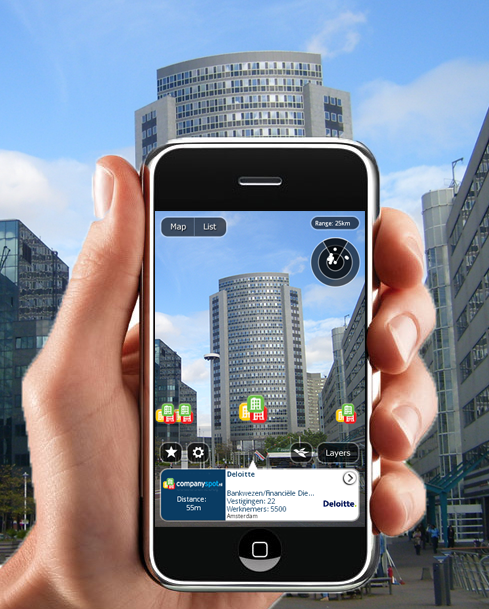
\includegraphics[scale=0.16]{images/AR_now}
\end{subfigure}
\begin{subfigure}{0.2\textwidth}
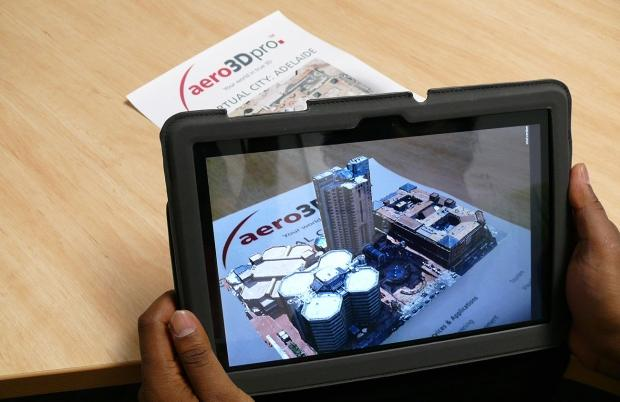
\includegraphics[scale=0.22]{images/AR_now1}
\end{subfigure}
\caption{AR in present smartphones}
\label{pic:arnow}
\end{figure}
     
\subsubsection{Digital Transparency}
One more motivation for this project come from the augmented reality (AR) in present smartphones. The AR is smartphones can majorly be classified into two types
\begin{itemize}
\item \textbf{Indirect AR} Figure \ref{pic:arnow} shows augmented reality applications in current smartphones. This gives the user a video see-through experience, as the view is from the camera's perspective.
\item \textbf{Direct AR} These are the systems that give a perspective from user's point of view and hence give more immersive experience than indirect AR system. Holo-lens and meta-glasses are examples of direct AR systems. 
\end{itemize}

\section{Method}
\subsection{3D Geometry of Problem}
    -Jenna. describe the vectors involved
\subsection{Multi-view Geometry}
    -Jai. - this is a overview, put equations here
\subsection{Face Detection}
    -Jenna, I'm assuming this is Viola-Jones
\subsection{Classifier}
    -Jai, not sure if this is needed.
\subsection{Inertial Measurement Unit}
    -Jenna
\subsection{Kalman Filter}
    -Jai
\subsection{Extended Kalman Filter}
    -Jenna
\section{Experiments}
\subsection{Multi-View Geometry Experiments}
    -Jai, make subsubsections as needed
\subsection{IMU Experiments}
    -Jenna, make subsubsections as needed
\section{Conclusions}
    -Jai
{\small{
\begin{thebibliography}{11}

\bibitem{BusinessInsider}
Yarow, Jay. "Here's Why Apple Made That Motion-Effect For The Background Of The New IPhone Software." Business Insider. Business Insider, Inc, 25 Sept. 2013. Web. 11 Dec. 2015.

\bibitem{DigitalTrends}
Pelegrin, Williams. "Why Isn’t the Fire Phone Truly 3D? Amazon’s ‘Dynamic Perspective’ Tech Explained." \textit{Digital Trends}. Digital Trends, 18 June 2014. Web. 11 Dec. 2015.
\end{thebibliography}

\end{document}

